\section{Data filtering}
\label{section: tracking method - data filtering}

One issue present with the mmWave Sensors (in our experience) is the fact that they are susceptible to both environmental noise as well as seemingly random noise. 
This noise often occurred in "streaks", lines of points through your 3d space. 
These "streaks" were not very dense spatially and usually only existed for a single frame, they often formed in the general shape of a line, though never exactly so, see \cref{figure: noise steak}.
Due to these attributes, a combination of a temporal as well as a spatial filter was used to filter out the noise points.

\begin{figure}
    \centering
    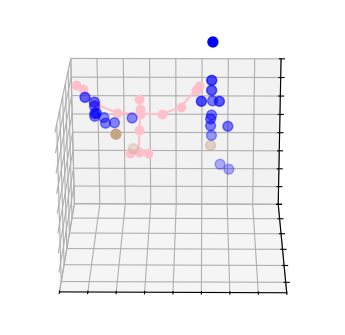
\includegraphics[width=0.5\linewidth]{figures/internal data/noise streak.png}
    \caption{A noise streak in the data (right-hand side of image)}
    \label{figure: noise steak}
\end{figure}

For this section, it's useful to know that the MMWave produces roughly 10 frames per second, thus each frame is roughly 100 ms.

\subsection{Spatial Filtering}
\label{sub-section: tracking method - data filtering - density filtering}

A very common strategy for filtering spatial data is to look at the density and internal cohesion between points.
The main idea on which this is based is the assumption that points with \textit{many close neighbors} are likely to \textit{represent reality well}, a "strength in numbers" kind of philosophy.
In our system, the \textit{spatial filter} looks on a \textit{frame by frame basis} at the clustering of the points.
Each point then gets assigned a value based on the cumulative weight of its neighbors (distance < 25 cm). 
Based on this value, points can be labelled as "noise" or "signal".

The main function of spatial filtering is to remove outliers, to always let large clusters pass, and to give an indication of how important any sparse clusters are.
By using the cumulative weight of the neighbours of a point, we also ensure that points which have already been shown to be more likely to be of use will be disproportionately selected.
One type of noise that the spatial filtering does not handle well, however, is dense but brief noise spikes, since our spatial filtering method only takes into account a single frame.
That is why the system also uses \textit{temporal filtering}.

% We also filter on the density in a single frame, since high in-frame consistency also often shows high quality of the data.
% However, sometimes noise streaks are dense enough to falsely trigger this system.


\subsection{Temporal Filtering}
\label{sub-section: tracking method - data filtering - temporal filtering}
The main function of the \textit{temporal filter} in this system is to provide stability across frames and to detect and remove noise spikes.
The temporal filter achieves this in a very similar way to the spatial filter, but instead of considering other points in the same frame, it only considers points in previous frames.
More specifically, the temporal filter takes into consideration the three frames (0.3-0.4 seconds) which came before, it then gives each point a score equal to the cumulative weight of spatially nearby points (within 20 cm) within these prior frames.
This means that points in a dense cloud may all get a very low score if little or no data has been found in that area recently.
In this way, the \textit{temporal filter} can 'punish' any inconsistent data, such as sudden but dense noise spikes.

Removing inconsistent data is not the only thing which the temporal filter does.
The temporal filter also 'rewards' points in a very stable area more than the density filter would, because the temporal filter takes into account points of three different frames.
This means that any data which is consistently present in an area across frames will be highly rated by the temporal filter, even though it takes into account a slightly smaller neighbourhood (20 cm as opposed to the 25 cm of spatial filters).
That being said, on their own, temporal filters can often miss large amounts of data, since the MMWave sensor does not always produce temporally consistent data, as discussed in \cref{sub-section: introduction - background - millimeter wave radar}.
That is why the actual system uses a combination of both a \textit{spatial} and a \textit{temporal} filter.


% Temporal data filtering was chosen, as the noise most often encountered was only present in a single frame. 
% By comparing the points in subsequent frames, these noise points can be filtered out by looking at the stability across frames.
% This was implemented by checking the number of neighbours on different frames that any point had within a specified distance (e.g., 10 cm). 
% In this case, even dense clusters on a single frame will be filtered out if this cluster is not present on other frames.
% 
% A danger of this approach is that you might lose correct points, this problem becomes more prevalent if the data is not always consistent over time.
% If the FMCW measures an arm (so not noise) in frames 1, 3, and 5, all that data will be discarded if we only consider a window of 3 frames (centred on the frame to be looked at, so on frame 3, we consider frame 2, 3, 4).
% Due to this side effect, it's important to choose the \textit{window of frames} you consider, as well as the \textit{minimum number of neighbours} and the \textit{distance within which you count as a neighbour}.


\subsection{Combined Filtering and Tuning}
\label{sub-section: tracking method - data filtering - combined filtering and tuning}

The system uses a combination of the \textit{spatial} and the \textit{temporal} filters, where it combines their respective scores, to make use of the strengths of both, while mitigating the weaknesses of both.
The combined filter has six variables which it can tune: the number of frames considered in the temporal system; for both the \textit{spatial} \textbf{and} the \textit{temporal}, the neighbourhood size considered, and the threshold cumulative weight to distinguish between noise an signal; and lastly the amount we take into account the spatial result or the temporal result.
Combining these two systems, however, does make it more difficult to tune, as there are more moving parts.
Therefore, a specific tuning strategy was thought up beforehand to get the system to a reasonable state. Afterwards, small tweaks were still made, based on what looked good to the visual inspection of the researcher.
% This is the main reason why we made a specific tuning strategy for this system before we started actually tuning it, though some manual tuning was still required in the end.

The tuning strategy which was used for this system was based on two principal ideas, namely, that the spatial filtering would be best at getting our positive values, while still avoiding some outliers and that the temporal filter would be able to provide enough of a counterbalance to mark inconsistent points as noise, while keeping the consistent points to be signal.
Our tuning strategy is thus to start by tuning the \textit{spatial filter} on its own in such a way that it captures all points we deem to be part of the signal, this means that it will also capture some points which are deemed to be noise (by the researcher).
Then the \textit{temporal filter} should be tuned, once again on its own, in such a way that it must not capture any noise, even if this means missing some points which are part of the signal.
These two filters are then combined (starting with a 50-50 split of effectiveness), and fine-tuning will happen. 
Here, the various variables will be modified slowly to resolve problems which are encountered.
In general, if signal points are missed, we should want either to increase the neighbourhood size of the spatial filter, lower its threshold, or make it more prevalent in the filter split.
In a similar vein, if noise points are not identified as such, we will want to increase the prevalence of the temporal filter in the filter split, lower the temporal threshold, or decrease its neighbourhood size.

A big advantage of this system is that it can be quickly tuned to the specific scenario, since the output of MMWave sensors can differ quite drastically based on the physical setup of the sensor and its environment.
This means that a system can be moved around with relatively little effort when you compare it to systems based on deep learning.
If you have a good quality metric for a point cloud recording, e.g. you want a lot of points and the points should be stable, you might even be able to automate it due to the low number of input parameters.

% Combined filters aim to make use of the best of both filters while mitigating the weaknesses of both filters.
% Tuning such a system is always an important part, the way this system was tuned was by first loosely tuning both systems, keeping in mind what we want from them.

% The density filter was tuned in such a way that it would recognise most actual hand recordings (with any significant number of points, e.g. 5-7 min) while letting through as few noise streaks as we can.

% The temporal filter was filtered in such a way that it notices a decent number of hand positions, while prioritising filtering out noise streaks.

% So density should catch almost all hands, while temporal should ignore almost all noise.

% During the combination of both filters, we want to give enough weight to temporal filter, to remove most noise streaks, but we want to not make it to great, so that we still recognize hand clusters which are only "good visible" in one frame.

% We tune the individual filters with Distance (for neighber search) and threshold neighber value. And for temporal, we also use the number of frames considered (values between 3-7 where considered, though any number > 5 (~half a second) already risks being more noise then data).
% Lastly we ofcourse have to decide in what manner we want to combine both.

% The advantage of doing it this way is that you can "retune" if you're tackeling a different scenario. e.g. a scenario with slow moving hands will probably want to consider a higher number of frames, while one with fast moving hands wants to consider less frames. So too you can make density filters more prevalent in your final filter if you don't encounter a lot of random noise, while you can lean more on temporal filters if you are.
